\chapter{An Adaptive Grasping Control Architecture for Whole Body Mobile Manipulation} \label{chapter_control}
Humans use eye and touch to monitor the entire process of grasping. They can change the grasping strategy on the fly when needed. This is why humans are capable of grasping objects very robustly. 
In this chapter, we address the problem of grasp execution and demonstrate how the grasping can be executed robustly under limited sensing capability.  

\section{Introduction}
Grasp execution is one of the most important steps for grasping success. Many earlier works use vision, tactile sensing, proximity sensing to improve the robustness of grasp execution (\cite{Felip2009},\cite{Hsiao2010},\cite{Hudson2012},\cite{jiang2012seashell}). Grasp execution on a real robot can be used to test whether the planned grasp configuration is feasible or not. Due to the error of object localization, sensor calibration and uncertain robot motion, the actual grasping configuration may differ from the planned one. Therefore, we need to handle these errors and keep the actual grasp configuration as close as possible to the intended one. 

Many approaches (\cite{Kamon1996},\cite{Rao2010},\cite{Roa2009}) which address the grasping problem usually assume perfect executions. They usually follow a sense-plan-action paradigm to execute a grasp. In the sensing phase, a robot recognizes, localizes and segments a desired object from the environment. In the planning phase, grasping points and grasping trajectory are calculated. In the action phase, the robot executes the  planned grasping trajectory to perform the grasp, usually in open-loop. One problem related to this paradigm is, sensing of object's state is missing in the action phase. If the action phase takes more than several seconds  without updating the object's state, the robot is unable to react to actuation error or external perturbation. Humans also use this paradigm to perform grasping but the sense-plan-action cycling time is much shorter. They maintain eye contact to the object until the object is fetched. In addition, they can adapt their grasp motion when object is displaced. In order to achieve maximal efficiency, humans seamlessly combine their locomotion, body, and arm movement for the entire grasping process.

In this chapter, we propose a flexible and adaptive grasping control architecture to imitate  human grasping. The flexibility is reflected in the freedom of choice and combination of  required actuators in different grasping phases. We define three grasping phases for the entire grasp execution process as shown in Fig.~\ref{fig:grasping_process}. During the initial phase, the gripper is far away from the object, so the robot can execute an arm and platform coordinated motion for approaching the object. In grasp motion phase, the gripper is closer to the object, the robot can stop the coordinated motion and use arm-only movement to reach the pre-touch configuration. In the force-closure phase, the robot can control the gripper and arm simultaneously so that grasping forces are applied in the 	normal direction. The control architecture enables the robot being adaptive during the grasp execution. The robot can continuously update an object's state and changes the corresponding grasp trajectory.  We evaluate the proposed control architecture on our robot in a challenging grasping task: grasping paper folded cylinder. To increase difficulty, we specially choose the sensor which has significant noise. This challenge can test whether the proposed architecture can handle light objects with limited perception capability. The experimental result shows that our approach can handle the challenging grasping tasks, and outperforms a traditional approach.  
\begin{figure}[!htbp]
\centering
\includegraphics[width=1\linewidth]{grasping_process.pdf}
\captionsetup{justification=raggedright}
\caption{A grasp execution process contains three intermediate grasping phases.}
\label{fig:grasping_process}       
\end{figure} 

\section{Related work}
A robust grasp execution requires continuous sensing. In general, two types of sensing can be found in the earlier works which address the grasp execution problem. During the reach-to-grasp phase, visual servoing is the primary method to guide the movement of gripper. Many works use the method (\cite{Kragic2002},\cite{Gridseth2015},\cite{Fujimoto2000}) for this task. During the force-closure phase, force and tactile sensing is the promising method to apply sufficient grasping forces to establish a stable grasp. Several works (\cite{Maekawa1996},\cite{Dang2012tactile},\cite{Dang2013}) use force or tactile sensing for grasp stability assessment and in-gripper manipulation. In addition to the sensor modality, we also give a short review on the control architecture and focus on the methods which allow whole body manipulation. 
 
\subsection{Methods using visual servoing} 
Visual servoing is primarily used in the reach-to-grasp phase, in which the gripper moves towards an object yet not in contact with it. Vahrenkamp et al.~\cite{Vahrenkamp2008} proposed a hybrid method that combines visual estimations with kinematically determined orientations to control the movement of a humanoid arm. They demonstrated how a robust visual perception is used to control complex robots without hand-eye calibration. Furthermore, they improve the robustness of their system  by estimating the hand position in case of failed visual hand tracking due to lightning artifacts or occlusions. 

\begin{figure}[!htbp]
\centering
\includegraphics[width=1\linewidth]{rw_visualservoing.png}
\captionsetup{justification=raggedright}
\caption{Methods using vision for grasp execution. (a) A method~\cite{Vahrenkamp2008} which combines visual perception and robot kinematics for determining motion of grasping. The approach was evaluated with the humanoid robot using the stereo system of the active head for perception as well as the torso and arms equipped with five finger hands for actuation. (b) A method~\cite{Gratal2012} which uses visual servoing on grasping unknown objects. The grasp motion is executed with open loop. (c) A method~\cite{Mansard2007} which allows grasping while walking for a biped humanoid robot.}
\label{fig:rw_visualservoing}       
\end{figure} 

Recatala et al.~\cite{Recatala2004} employed a stereo camera and a two finger gripper with an eye-in-hand configuration to study visual guided grasping. Their system tracks a pre-defined grasping points in image space and use that for the control law. The tracking is based on using an invariant description with respect to the object.   

Different from the above methods which only consider visual servoing of one robot, Muis et al.~\cite{Muis2005} exploit two robots and demonstrate how a robot with eye-to-hand configuration and another robot with eye-in-hand configuration can improve the tracking performance. The drawback of each configuration is resolved by the benefit of the other.  

Traditionally visual servoing can only also be applied to tracking objects with an existing model. Gratal et al.~\cite{Gratal2012} proposed a grasp pipeline which exploits visual servoing also on unknown objects. They demonstrated how visual servoing can be both applied for offline calibration and online grasp execution. 

Visual servoing has also been applied to humanoid robots for grasping on the move. Mansard et al.~\cite{Mansard2007} proposed a framework for building complex whole-body control and realized visually-guided grasping while walking on a humanoid robot. They divide the control into several sensor-based control tasks. This structure enables a very simple access for task sequencing and task-level control.

We also use visual sensing for guiding the gripper towards objects. The methods which discussed so far do not consider the uncertainty of a tracking result, so their methods can not react to the tracking uncertainty. Different from these methods, our architecture employs uncertainty of tracking to generate new grasps for adaptation. Therefore, our approach is able to generate the grasp which maximizes the success probability at each time cycle.    

\subsection{Methods using force sensing} 
As long as the robot touches an object, force sensing becomes a promising way for a robust grasp execution. Typically, force sensing refers to measuring joint torque or fingertip pressure. Kazemi et al.~\cite{Kazemi2012} proposed force compliant motion primitives to handle small objects. They exploited strain gauges on the joint of a gripper to detect collision with the support plane of the object. After collision is detected, fingers are closed using a control scheme that enables fingertips to slide on the support surface. Pastor et al.~\cite{Pastor2011} presented an approach for generating contact reactive grasp motion using previous sensor experiences. These knowledge are acquired from human demonstrations. They exploit DMPs \cite{Ijspeert2013} to generate adaptive trajectories based on tactile and force torque sensing.  

\begin{figure}[!htbp]
\centering
\includegraphics[width=1\linewidth]{rw_forcesensing.png}
\captionsetup{justification=raggedright}
\caption{Methods using force sensing for grasp execution. (a) In~\cite{Pastor2011}, the robot is first demonstrated how to grasp an object using kinesthetic teaching. At test time, the robot detects object displacement with strain gauge mounted on the gripper and adapts its grasp motion to a new object position. (b) A force compliant motion primitives is proposed in~\cite{Kazemi2012}. A coordinated lift motion and close motion ensures the gripper always maintains contact with a support plane. This method works well for flat objects lying on a horizontal plane. (c) A method for in-hand grasp adaptation proposed in~\cite{Li2014}. A three-finger initial grasp is first established on an object. The position of one finger can be changed online to maintain the stability of the grasp, when the weight of the object is increased. }
\label{fig:rw_forcesensing}       
\end{figure}

Tactile sensing is another commonly used strategies for establishing the final grasp (\cite{Dang2014},\cite{Dragiev2013},\cite{Laaksonen2012},\cite{jiang2012seashell}). Romano et al.~\cite{Romano2011} proposed a grasp controller based on tactile pressure and accelerometer to generate robotic tactile signals to mimic human SA-I, FA-I, and FA-II channels. These signals are used to indicate a set of event transitions between Close, Load, Lift and Hold actions of the gripper. The controller selects appropriate initial forces and increases or decreases as needed to prevent an object from slipping or determine when to set it down. The proposed controller is implemented on a parallel gripper. 

Tactile sensing can be also used for grasp adaptation with multi-finger grippers. Li et al.~\cite{Li2014} proposed a grasp adaptation strategy for a multi-finger gripper. The method is able to handle the uncertainty of object's physical properties. A stability estimator was proposed to judge when to apply a grasp adaptation of a new grasp. The new grasp is chosen by the similarity of training examples. 

In this chapter, force sensing is not considered as the primary sensing modality, because the stiffness of the target objects that we choose are extremely small. The tactile sensor is not sensitive enough to measure the grasping force. Instead we focus us in the reach-to-grasp stage, and use vision as our primary sensing modality. 


 
\subsection{Methods considering whole body coordination}
In addition to the sensing modalities we reviewed so far, how to combine the sensing modality into a control architecture has also been addressed by many researchers. Here, we focus on the work for tasks requiring whole body coordination.

 Back in the middle of the 90's, Khatib et al.~\cite{Khatib1996} proposed a task-oriented control method for dynamic mobile manipulator coordination, in which a decentralized control structure was used to perform cooperative tasks with multiple mobile manipulators. Their focus is not on performing manipulation tasks like e.g. grasping.

Many work exploit arm-platform coordination in order to execute tasks such as `opening doors', because a static robot can not perform such tasks due to the limited arm workspace. Ott et al.~\cite{Ott2005} used a mobile manipulator which has a 7-DOF arm and a omni-directional base to perform the door opening task. Based on impedance control, they generated the required arm-base coordinated motion for door opening, without knowing the door size and an explicit opening trajectory. During the operation, the robot arm kept the door at a certain distance while the base moved through the door. In \cite{Chitta2010}, a framework for planning door opening trajectory with arm-base coordination was presented. They used a graph-based planning approach that allows a robot can open various doors both by pushing or pulling. Both of the work focused on how to use arm-base coordination to perform door opening trajectory. How to establish the grasp to the handle of the door is however not addressed.  

\begin{figure}[!htbp]
\centering
\includegraphics[width=1\linewidth]{rw_control.png}
\captionsetup{justification=raggedright}
\caption{Tasks that require tight coordination in between the motion of
the base and the motion of the arm. (a) In~\cite{Ott2005}, a mobile manipulator equipped with a single arm performs door opening task. Cartesian impedance controller was proposed to control the elastic joints of the arm. (b) A graph search-based motion planning method~\cite{Chitta2010} is proposed to plan trajectories for door opening. The method is able to handle a variety of door types. (c) A reactive whole-body control mechanism~\cite{Dietrich2011} for a torque controlled robot. The control method can be used for  performing tasks such as catching a flying ball~\cite{birbach2011realtime}. }
\label{fig:rw_control}       
\end{figure}

Collision avoidance for mobile manipulators is also a common topic addressed
by many authors. Omrcen et al.~\cite{Omrcen2003} proposed a method for real time obstacle avoidance using a torque and velocity controlled mobile manipulation robot. High compliance of the arm ensures safety without using any sensors. Dietrich et al.~\cite{Dietrich2011} proposed a reactive whole-body control mechanism for controlling a mobile manipulation robot with very high degree of freedom. They integrate several control requirements into a task hierarchy. These approaches demonstrate how to use arm-base coordinated motion to expand the robots' workspace. 

Our control architecture not only covers many aspects which are also existed in the previous work such as collision avoidance, coordination of actuators, but also seamlessly integrates vision feedback which may contain information of perception uncertainty. In addition, our architecture also monitors and controls switching of grasping phases to guarantees subgoals of grasping phases are subsequently reached for ensuring the final success.

\section{Contributions}
The main contribution of this chapter is the adaptive grasp control architecture. Different from the previous work which usually only address a sub-process of grasp execution. The control architecture monitors and controls the entire grasping process, from the phase that an object is detected to the phase the final grasp is established. The entire grasping process is decomposed into three phases. The robot has the freedom to choose a different combination of actuators to execute the motion in each phase. A tight coordination in between arm, base, and gripper imitates how a human performs grasping. 

Different from previous work, vision feedback as well as the uncertainty of the feedback can be integrated into the system so that our system can adapt to uncertainty and external perturbation. An uncertainty-aware grasp configuration can be updated in each control cycle according to the vision feedback. We evaluate the complete system with a challenging grasping tasks. By comparing with two traditional approaches, our method achieved the highest grasping accuracy of the experiment. 


\section{System architecture}
We propose a system architecture depicted in Fig.~\ref{fig:adaptive_control_architecture} for adaptive grasping control. The system architecture is designed to close the perception-action loop.  The entire loop begins with the processing of sensor data. The component `Tracker' estimates the state of an object based on the sensor data. The output of this component is a belief distribution of the object state. Then, the component `grasp synthesis' takes the perception result and generates a set of grasp configurations. These include the afore-defined pre-grasp, pre-touch and force-closure poses. The component `Grasp phase control' monitors the current state of the robot and generates goal configurations where the gripper of the robot must reach. The motion adaptation takes the TCP and the grasp posture configurations as input and generates trajectories for a gripper.   The output of Motion adaptation consists a TCP trajectory and a grasp trajectory. The TCP trajectory defines the 6D path and velocity of the gripper, while the grasp trajectory defines the postures of the gripper. Since we represent the posture in a low dimensional space of a gripper, the actual finger joint to be executed has to be calculated by the `Gripper posture generation.' To execute a TCP trajectory, the component `Redundancy resolution' is used. It converts the velocity in task space to that in joint space. The output of the `Redundancy resolution' and the `Gripper posture generation' are both joint velocities. The component `whole body coordinated control' takes the joint velocities as input and generate the corresponding hardware control signals to the robot.


\begin{figure}[!htbp]
\centering
\includegraphics[width=0.9\linewidth]{controlarchitect.pdf}
\captionsetup{justification=raggedright}
\caption{System architecture}
\label{fig:adaptive_control_architecture}       % Give a unique label
\end{figure}   




\subsection{Motion adaptation}
\paragraph*{Adaptation of TCP Cartesian trajectory}
In this grasping scenario, the robot has to adapt its grasp to the measurement online. In order to achieve online motion adaptation, we choose dynamic movement primitives (DMPs) to generate the grasp motion. DMPs were originally proposed by Ijspeert et al. \cite{Ijspeert2013} and Pastor et al. \cite{Pastor2011} to learn trajectories from human demonstration. After learning, DMPs allow generalizing the learned path to new goal configurations. We represent the grasp motion using Cartesian trajectory. Two steps are required to generate the trajectory. The first step is learning the characteristic of a reference trajectory \footnote[1]{also called demonstration trajectory in the context of learning by demonstration}. The second step is the adaptation from the reference trajectory. 
The reference trajectory is represented by a set of discrete points, which can be obtained using e.g. kinesthetic teaching  \cite{Herzog2012}. As there is no human demonstration in our setup, we generate the reference trajectory using a cubic spine. The spline is generated by taking a current robot pose, a pre-grasp and a pre-touch configuration as input parameters. A DMP in one-dimensional (1-D) space is formulated by two differential equations which are equivalent to a non-linear mass-damper system:

 \begin{align}
  \label{equ:tauv}
 \tau \dot{v} &= k\cdot({g}-x^{\text{dmp}}) - d \cdot v + (g- {x}^{\text{dmp}}_0) f(s)  \\
 \label{equ:tauxv}
  \tau \dot{x}^{\text{dmp}} &= {v},
 \end{align}
where $x^{\text{dmp}}$ denotes the position of a 1-D DMP system. ${x}^{\text{dmp}}_0$ is the start position and $g$ is the position in which the DMP system converges.  $k$ and $d$ denote stiffness and damping. $f(s)$ is an non-linear function for approximating arbitrary convergent characteristics. $f(s)$ can be realized by a linear combination of a set of basis functions. $s$ is a phase variable with $s \in [0,1]$ and is determined by the following canonical system
\begin{equation}
 \tau \dot{s} = - \alpha s.
 \label{equ:canonicalsys}
\end{equation}
$\tau$ is a time-scaling parameter used to scale the length of the trajectory to be generated. The process of learning a reference trajectory include: (1) Compute the velocity of the reference trajectory for each time stamp. (2) Compute the phase parameter $s$ of the i-th point by 
\begin{equation}
 s_i = e^{- \alpha / \tau \cdot t }
 \label{equ:compute_phase}
\end{equation}
(3) Compute the target value $f_{\text{target}}(s_i)$ for each point on the reference trajectory by plugging the points and velocities into Eq.~\ref{equ:tauv} and \ref{equ:tauxv}. (4) Use linear regression to estimate the parameters of $f(s)$.

For learning the position of a reference TCP trajectory, three instances of a 1-D DMP system are required to represent each dimension in a cartesian space. However, the orientation of the reference TCP trajectory can not be directly represented by three 1-D DMP system if we choose Euler angles to represent the orientation, as the Euler angles contain singularity at $2\pi$. Instead, we use quaternion to represent the orientation so that a single quaternion-based DMP system proposed in \cite{Pastor2011} can be used to learn the orientation characteristics of the TCP reference trajectory. 

\begin{figure}[!htbp] 
\centering
\begin{subfigure}[t]{.3\linewidth}
  \centering
  \includegraphics[width=1\linewidth]{figure/dmp_origin.png}
  \caption{Reference trajectory}
  \label{fig:sub1}
\end{subfigure}
\begin{subfigure}[t]{.3\linewidth}
  \centering
  \includegraphics[width=1\linewidth]{figure/dmp_goal_changed.png}
  \caption{Trajectory adaptation on new goal configuration }
  \label{fig:sub2}
\end{subfigure}
\begin{subfigure}[t]{.3\linewidth}
  \centering
  \includegraphics[width=1\linewidth]{figure/dmpdmpchanged_explanation.png}
    \caption{Overlap of reference trajectory  and adapted trajectory.}
  \label{fig:sub3}
\end{subfigure}
\caption{An example of trajectory adaptation using DMPs}
\label{fig:dmp_example}
\end{figure}

Generate a new trajectory from a learned DMP system include following steps: (1) Calculate the phase parameter $s$ using Eq.~\ref{equ:compute_phase} for a  given time stamp $t$. (2) Evaluate the function approximator $f(s)$ and compute $\dot{v} $ and $\dot{x}^{\text{dmp}} $. (3) Compute a new trajectory point by 
numeric integration with 
 \begin{align}
x^{\text{dmp}} (t+\delta t) &= x^{\text{dmp}}(t) + \dot{x}^{\text{dmp}}  \cdot \delta t \\
v (t+\delta t)&= v(t) + \dot{v} \cdot \delta t
\label{equ:numeric_integration}
\end{align}
where $\delta t$ is a very small time duration. We choose $\delta t$ to be 1 ms to reach a sufficient accuracy. To generate the whole trajectory, Step 1 to 4 is then repeated until $g-x^{\text{dmp}}$ is under a threshold. At an arbitrary time stamp, if a new goal configuration of TCP is available, we can plug it into Eq.~\ref{equ:tauv} to force the DMP system converge to the new configuration. In this way, the grasp motion to be executed is adapted to new sensor measurements.      Fig.~\ref{fig:dmp_example} explains the adaptation of cartesian trajectory on a new goal configuration.


\paragraph*{Adaptation of low-dimensional grasp trajectory} 
Similar to adaptation of a cartesian trajectory in the `grasp-motion' phase, we also employ DMPs to generate trajectories for the `force closure' phase. An example force closure trajectory is shown in Fig.~\ref{fig:force_closure_traj_alone}. The force closure trajectory contains a closing movement of fingers and a lifting movement of the gripper. In this way, the gripper realizes the same closing behavior of a parallel gripper to ensure the desired contact region of the finger moves anti-parallel towards each other. 

\begin{figure}[!htbp]
\centering
\includegraphics[width=0.3\linewidth]{force_closure_traj_alone.png}
\captionsetup{justification=raggedright}
\caption{A reference trajectory for learning coordinated force closure motion.}
\label{fig:force_closure_traj_alone}       % Give a unique label
\end{figure}   

We realize the grasp trajectory with two DMP subsystems which are synchronized using the same DMP phase parameter $s$. One DMP subsystem generates the desired lifting trajectory while the other DMP subsystem generates a low-dimensional finger trajectory of the gripper. In section \ref{sec:gripper_parametrization}, we propose a method for parameterizing a high DOF gripper by using the `Eigengrasp' concept. The method reduces the total DOF of a gripper to the number of joint groups that we defined for that gripper.  For the gripper we use in this work, we need totally four one-dimensional DMPs to represent the closing trajectory, because four joint groups are defined for the Schunk gripper. The entire joint movement of the gripper is calculated according to Eq.~\ref{equ:eigen_grasp} by the module `Gripper posture generation.'



\subsection{Arm platform redundancy resolution}
In order to control motion in cartesian space, the Cartesian trajectory generated by DMPs must be converted to the motion controls in joint space. For robots which have more than six DOF,  the joint redundancy can be exploited. We apply the idea of nullspace optimization \cite{Nakanishi2005} to resolve the redundancy. Let $\underline{{x}_d}$ be the desired position and orientation of tool center point (TCP), and let $\underline{q_d}$ denote the desired joint positions. The desired joint velocity $\dot{\underline{q_d}}$ can be expressed by 
\begin{equation}
 \dot{\underline{q_d}} = \underline{J}^+ \dot{\underline{x_d}} + (\underline{I} - \underline{J}^+  \underline{J} )\underline{\xi},
\end{equation}
where $\underline{J}^+$ represents the pseudo-inverse of Jacobian $\underline{J}$  that is defined by $\underline{J}^+ = \underline{J}^T(\underline{J}\underline{J}^T)^{-1} $. The term $(\underline{I} - \underline{J}^+  \underline{J} )$ projects an arbitrary vector $\underline{\xi}$ onto the nullspace of Jacobian. In this work, we exploit three criteria to resolve redundancy, which are generally applicable to any kind of mobile manipulation robots. These criteria are self collision avoidance, joint limit avoidance and singularity avoidance. We define each criterion as a unique cost function of joint position ${E}^i(\underline{Q})$. By setting $\underline{\xi} = -\nabla(\sum\limits_{i=1}^3 {E}^{(i)}(\underline{Q}))$, nullspace velocity reduces the total cost in the gradient direction.

%\subsubsection{Optimization criteria}
\paragraph{Self collision avoidance} This criterion ensures that a robot does not collide with itself. The gradient of cost function for self collision avoidance is defined by 
\begin{equation}
\label{equ:criterion1}
\nabla E^{(1)}(\underline{Q}) = \sum\limits_{(i,j)\in CP} \dfrac{ \text{d}E^{(1)}}{\text {d}D_{(i,j)}} \cdot \dfrac{\text{d}D_{(i,j)}}{\text{d}\underline{Q}},
\end{equation}
where $D_{(i,j)}$ denotes the distance between two links, which can potentially collide with each other. We compute link distances by means of the approach proposed in \cite{Larsen1999}. The gradients of link distances with respect to joint positions are computed numerically. $\dfrac{ \text{d}E}{\text {d}D_{(i,j)}}$ denotes the gradient of cost with respect to a link distance.   

\paragraph{Joint limit avoidance} This criterion ensures that the limits of the joints will not be overshot. Each joint of arm must work in a specified joint range. Overshooting of joint limit can cause hardware defects. The gradient of joint limit avoidance is expressed by 
\begin{equation}
\nabla E^{(2)}(\underline{Q}) = \left[\dfrac{\text{d}E^{(2)}}{\text{d}Q_1},\cdots,\dfrac{\text{d}E^{(2)}}{\text{d}Q_\text{N}}\right]^\text{T}.
\end{equation}
The cost function of each joint $E(Q_i)$ is defined as follows
%\begin{equation}
%{E^{(2)}}(Q_i) = \left\{
%\begin{array}{ll} \alpha_i \cdot \left[Q_i - ( Q_i^{\text{max}} -   Q_i^{\text{soft}}) \right]^2, & Q_i \in (Q_i^{\text{max}} -   Q_i^{\text{soft}} , Q_i^{\text{max}} ) \\
%         0 & \text{else}, \end{array}\right.
%\end{equation}
\begin{equation}
  E^{(2)}(Q_i) = \alpha_i \cdot \left[Q_i - ( Q_i^{\text{max}} -   Q_i^{\text{soft}}) \right]^2,
\end{equation}
where  $\alpha_i$ is a parameter to scale cost function. $Q_i^{\text{max}}$ denotes the maximum limit that joint $i$ can reach. $Q_i^{\text{soft}}$ is the range in which cost is activated.   
%\alpha_i \cdot \left[Q_i - ( Q_i^{\text{max}} -   Q_i^{\text{soft}}) \right]^2
\paragraph{Singular configuration avoidance} This criterion ensures that no singular configurations will occur during the whole grasping procedure. 
Near singular configuration small actuator torques will lead to a large end-effector wrench. This could cause jerk movement and overshoot hardware limitation. An approach to avoid singular configurations is to maximize manipulability defined by  
$M(\underline{Q}) = \sqrt{ \text{det}( \underline{J} \cdot \underline{J}^\text{T})}$. Similar to the first cost function (equation (\ref{equ:criterion1})), the gradient of cost for singularity avoidance is given by 
\begin{equation}
 \nabla E^{(3)}(\underline{Q}) = \dfrac{ \text{d}E^{(3)}}{\text {d}M} \cdot \dfrac{\text{d}M}{\text{d}\underline{Q}}.
\end{equation}

\subsection{Whole-body coordinated control}
A mobile manipulator is composed of individual hardware components. Each one has its interface for control. The   purpose of this module is synchronization of devices for executing trajectories containing high DoF. The structure of whole body coordinated control is depicted in Fig.~\ref{fig:coordinated_control}. The input of `Whole body coordinated control' is `Redundancy resolution', `Joint space motion planner', and `Gripper posture generation'. One use case is to control an arm and a platform simultaneously, we can use either the `Joint space motion planner' or the  `Redundancy resolution' to generate joint velocities.  As we did in chapter~\ref{chapter4}, for all collision-free motions, we use joint space motion planner to move the robot. In this chapter, we concentrate in grasp-motion phase. Typically, the robot approaches a pre-touch configuration of an object linearly, in this case, we use `Redundancy resolution' to convert a linear Cartesian trajectory to joint velocities. Another use case is to control an arm and a gripper simultaneously, we need `Gripper posture generation' to convert a low-dimensional gripper trajectory to the trajectory containing the entire joint positions using equation~\ref{equ:eigen_grasp}. We can generate a Cartesian trajectory of a gripper and a posture trajectory of each gripper joint to realize a coordinated grasping trajectory during force closure. The coordinated grasping trajectory is specially designed for grasping from the top of a flat object, so that during force closure phase a contact force is always maintained between the fingers and a support surface.   

The `Whole body coordinated control' contains two layers. The first layer is command allocation. The command allocation first splits the output of a high DoF trajectory and then it assigns joint velocities of the trajectory to each component. The second layer contains a set of low-level controllers. The low-level controllers convert the joint velocities to the commands accepted by the devices. For example, in order to control a base platform, the base controller must convert the joint velocities to linear and rotational velocities using equation~\ref{equ:velocity_conversion}. To control an arm, `arm controller' must first integrate the velocities to positions and then send the positions to the hardware. To control a gripper, a `Gripper controller' is proposed to send the desired velocities to each joint and stop the joints if the pressure measured by tactile sensors is higher than a pre-defined threshold. 

\begin{figure}[!htbp]
\centering
\includegraphics[width=1\linewidth]{armbasecontrol.pdf}
\captionsetup{justification=raggedright}
\caption{Whole body control architecture}
\label{fig:coordinated_control}       % Give a unique label
\end{figure}   

%\section{Control in force-closure phase}

%\subsection{Arm-hand coordinated control}

\section{Use case: grasping cylindrical objects with unknown dimension}
In this section, we choose another class of grasping problems to demonstrate the proposed system. How can a robot be able to conduct robust grasping, even the sensor used for perception has large noise. In chapter \ref{chap:grasplimitsensing}, we proposed a paradigm to deal with this situation. The main idea of this paradigm is to integrate the sensor measurement online and adapt control trajectories in an iterative fashion. The proposed system architecture provides the foundation to realize the paradigm. In order to demonstrate the proposed system architecture in this grasping scenario, we choose objects, the shape of which can be approximated by a cylinder, as target objects. We also assume that the target objects stand  upright on a support plane. This assumption simulates the most stable orientation of the cylindrical objects such as mugs, glasses and etc in the real world. 
Based on this assumption, the grasp can be easily parameterized to satisfy a task constraint. For example, if the robot is desired to perform a pouring task, the grasp configuration has to be parameterized so that the robot approaches and grasps the object from the side. In the following, we elaborate two necessary components to use the proposed system architecture, the first is tracking of object state and the second is grasp synthesis for cylindrical objects.   
 

\subsection{Measurement model for object state estimation} 
The shape of a cylindrical object can be represented by two parameters: radius and height. Since objects are placed in upright positions in this grasping scenario, we define additional two parameters to represent the position of the object. Since we require the robot to grasp from the side of an object, the height of the gripper can be chosen at the half height of the object. Thus, the height parameter is not the crucial parameter which affects grasp success. In contrast, the radius and the position of an object are the critical parameters which must be estimated accurately. Therefore, we only need to online estimate the radius and the position in this grasping scenario. We propose to use an extended Kalman Filter (EKF) for this task. The EKF is a method for state estimation. In order to use the EKF, a system model and a measurement model must be provided. In our case, the system model defines the distance covered by a gripper during a grasping process. The distance traveled by the gripper can be obtained from the odometry and the joint positions of a  robot's arm. The measurement model calculates desired measurements given the true state of a system. In the following we elaborate how the measurement model is defined for the given grasping scenario. 

\begin{figure}[!htbp]
\centering
\def\svgwidth{0.7\linewidth} 
\input{figure/cylindericalobject.tex}
\captionsetup{justification=raggedright}
\caption{A circular object measured by a sensor. $p_1$ and $p_2$ are the measurements used in EKF for estimating the position and the radius of the object.}
\label{fig:illustrate_measurement_model}
\end{figure}	

Without constraining the actual sensor we use for the grasping task, we assume the input data of the sensor can be converted to a data type of a laser scan. A laser scan is defined by a set of points in the polar coordinate system ($\underline{d}, \underline{\theta}$), where $\underline{d}$ is an array which gives a set of range measurements. $\underline{\theta}$ is also an array which has the same size as $\underline{d}$. Each $\theta_i$ in $\underline{\theta}$ defines the bearing angle for the corresponding range measurement  ${d_i}$. If the real sensor outputs a stream of point clouds, we can extract the 3D coordinate of the points on the plane that we interested and then convert them to the polar coordinates. In order to estimate the radius and the position of an object, we only need two critical points as a measurement. These two points hit two tangential lines of a circular object as shown in Fig.~\ref{fig:illustrate_measurement_model}. We define these two points as the measurement to be used in an EKF. By considering the triangular relationship, the desired measurement can be formulated by 
\begin{align}
\underline{z}_{\text{EKF}} &= \begin{bmatrix}
\underline{z}_{p_1}
\\ 
\underline{z}_{p_2}
\end{bmatrix} \\
&= \begin{bmatrix}
d_1 \\
\theta_1 \\
d_2 \\
\theta_2  
\end{bmatrix} \\
&= \begin{bmatrix}
 \sqrt{x^2_c +y^2_c -r^2_c} \\
  \text{atan2}(y_c,x_c) + \text{asin} ( \frac{r_c}{\sqrt{x^2_c +y^2_c} } ) \\
 \sqrt{x^2_c +y^2_c -r^2_c} \\
  \text{atan2}(y_c,x_c) - \text{asin} ( \frac{r_c}{\sqrt{x^2_c +y^2_c} } ) \\
\end{bmatrix},
\end{align}
where $(d_1, \theta_1)$ and $(d_2, \theta_2)$ are the desired measurement in polar coordinate of point $p_1$ and point $p_2$. $\underline{x}_o = (x_c , y_c ,r_c)$ denotes the position and the radius of the object in Cartesian coordinate of the sensor.

\subsection{Grasp synthesis for circular objects}
We use the same grasp success model proposed in \ref{sec:grasp_success_model} to evaluate the success probability of a grasp. The object is represented by its radius and position $\in \mathcal{R}^2$. A parallel gripper is chosen to grasp the object. The gripper configuration $\mathcal{G} \in \mathcal{R}^4$ contains the 2D positions of the left finger and the right finger. In order to validate the conditional grasp success model, we generate many random gripper configurations. For each configuration, we evaluate the conditional grasp success probability. Fig.~\ref{fig:circular_grasp_success}(a) depicts 10 random gripper configurations, the grasp success probability of which are higher than 90~$\%$. Fig.~\ref{fig:circular_grasp_success}(b) shows 10 negative examples, the conditional grasp success probability of which are lower than 10~$\%$. 

\begin{figure}[!htbp]
\centering
\def\svgwidth{1\linewidth}
\input{figure/grasp_success_circular.tex}
\caption{(a) Ten random sampled good pre-touch configurations, where the grasp likelihood larger than 0.9, (b) Ten random sampled bad pre-touch configurations, where the grasp likelihood smaller than 0.1.}
\label{fig:circular_grasp_success}
\end{figure}	 

The goal of grasp synthesis is to find an optimal pre-touch configuration.  The optimal pre-touch configuration is found according to equation \ref{eq_g_opt} by searching the maximal marginal grasp probability. Since the dimension of object state for a circular object is only three, we can integrate the equation \ref{e_grasp_success} numerically. The posterior of the object is obtained from the EKF estimation. It is represented by a multi-variate Gaussian $p(\underline{x}_o|\mathcal{Z}) = \mathcal{N}(\mu, \Sigma)$  where $\mu$ is a mean and $\Sigma$ is a covariance matrix. We integrate over the $\pm3\sigma$ interval to approximate the integral of equation \ref{e_grasp_success} by 

\begin{equation}
\begin{split}
 \text{P}(S | \mathcal{G} ,\mathcal{Z}) 
    &= \int_{\underline{x}_o} \text{P} (S | \underline{x}_o, \mathcal{G} )\cdot p(\underline{x}_o|\mathcal{Z}) d\underline{x}_o \\
    &=  \int_{\underline{x}_o} \text{P} (S | \underline{x}_o, \mathcal{G} )\cdot \mathcal{N}(\mu, \Sigma) d\underline{x}_o  \\
    &\approx \int_{\mu_1 - \sigma_1}^{\mu_1 + \sigma_1} \int_{\mu_2 - \sigma_2}^{\mu_2 + \sigma_2} \int_{\mu_3 - \sigma_3}^{\mu_3 + \sigma_3} \text{P} (S | x_{o},  \mathcal{G} )\cdot \mathcal{N}(\mu, \Sigma) \,  \text{d}x_{c} \, \text{d}y_{c} \, \text{d}r_{c}, 
\label{e_grasp_success}
\end{split}
\end{equation}
where $x_{1}, x_{2}, x_{3} $ represent the radius and the positions, $\mu_1, \mu_2, \mu_3$ are the means of positions and the radius. $\sigma_1, \sigma_2, \sigma_3$ are the diagonal elements of the covariance matrix $\Sigma$. In this case, we use Subplex~\cite{Rowan1990} implemented in NLopt~\cite{Johnson2010} to find the maximal probability of $\text{P}(S | \mathcal{G} ,\mathcal{Z})$. Fig.~\ref{fig:object_posterior_sample} visualizes a synthetic posterior distribution   with $\mu = (0, 0 , 0.01)$ and $
\Sigma = 
\begin{pmatrix}
0.01 & 0.008  & 0 \\ 
0.008 & 0.01  & 0 \\
0 & 0  & 0.01
\end{pmatrix}
$. The optimal pre-touch configuration for this posterior is depicted in Fig.~\ref{fig:optimal_pre_touch_conf}. The marginal success probability of this object posterior by taking the optimal pre-touch configuration is equal to $44.9 \%$. The absolute mass of probability depends on how the parameters are chosen for evaluating the conditional success grasp probability. Since the parameters we choose for calculating the conditional success grasp probability for this example is conservative, the success probability by taking the optimal pre-touch configuration is not high. However, the pre-touch configurations computed using our model are very close to the optimal in reality. From the figure we can see, that the grasp is explicitly computed for the given object state uncertainty. 
\begin{figure}
    \centering
    \begin{subfigure}[b]{0.45\textwidth}
        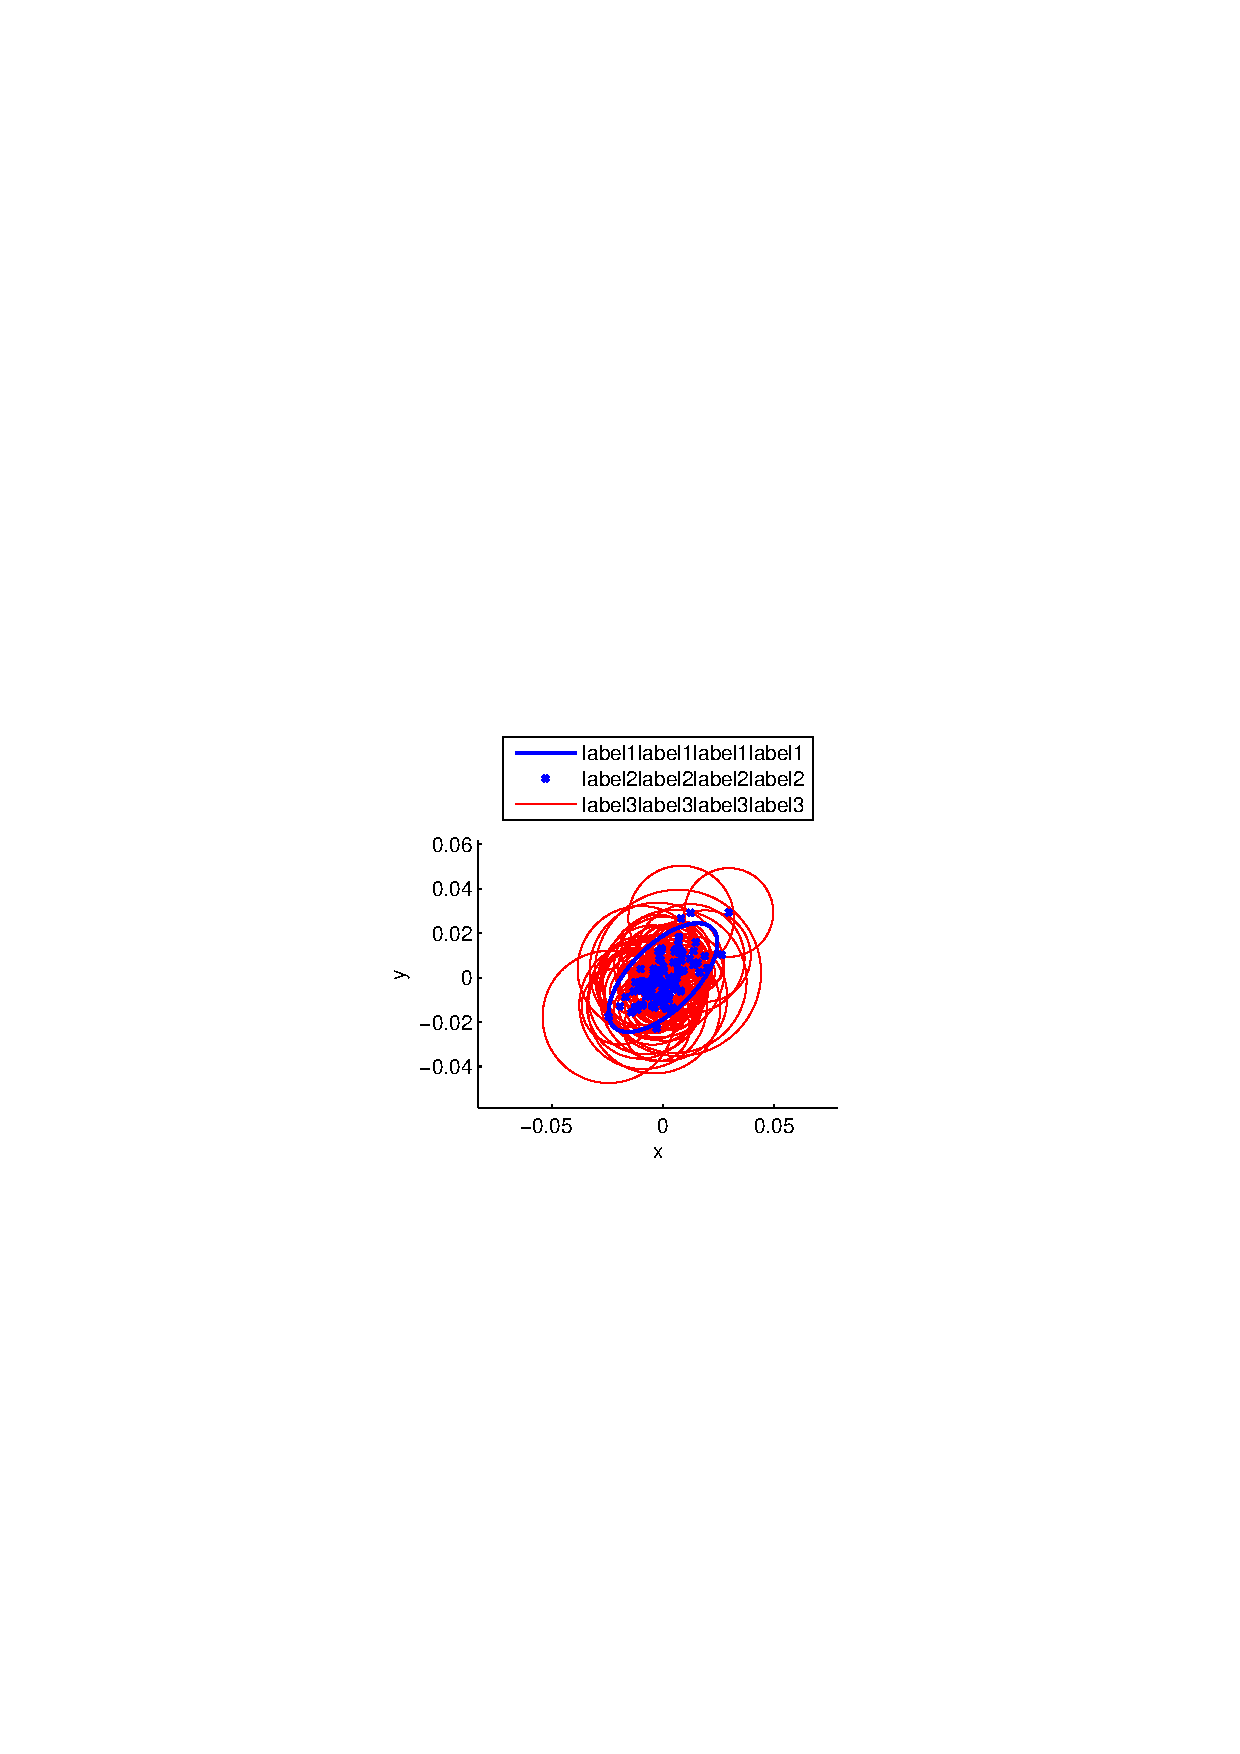
\includegraphics[width=\textwidth]{object_posterior_sample.pdf}
        \caption{A synthetic object posterior $p(\underline{x}_o|\mathcal{Z} = \mathcal{N}(\mu, \Sigma)$ where $\mu = \left( 0.01,0,0  \right) $ and $\Sigma$ is a covariance matrix with $\sigma_x = \sigma_y = \sigma_r = 0.01$ , $\sigma_{xy} = 0.008$ and $\sigma_{rx} = \sigma_{ry} = 0$ }
        \label{fig:object_posterior_sample}
    \end{subfigure}
    ~ %add desired spacing between images, e. g. ~, \quad, \qquad, \hfill etc. 
      %(or a blank line to force the subfigure onto a new line)
    \begin{subfigure}[b]{0.45\textwidth}
        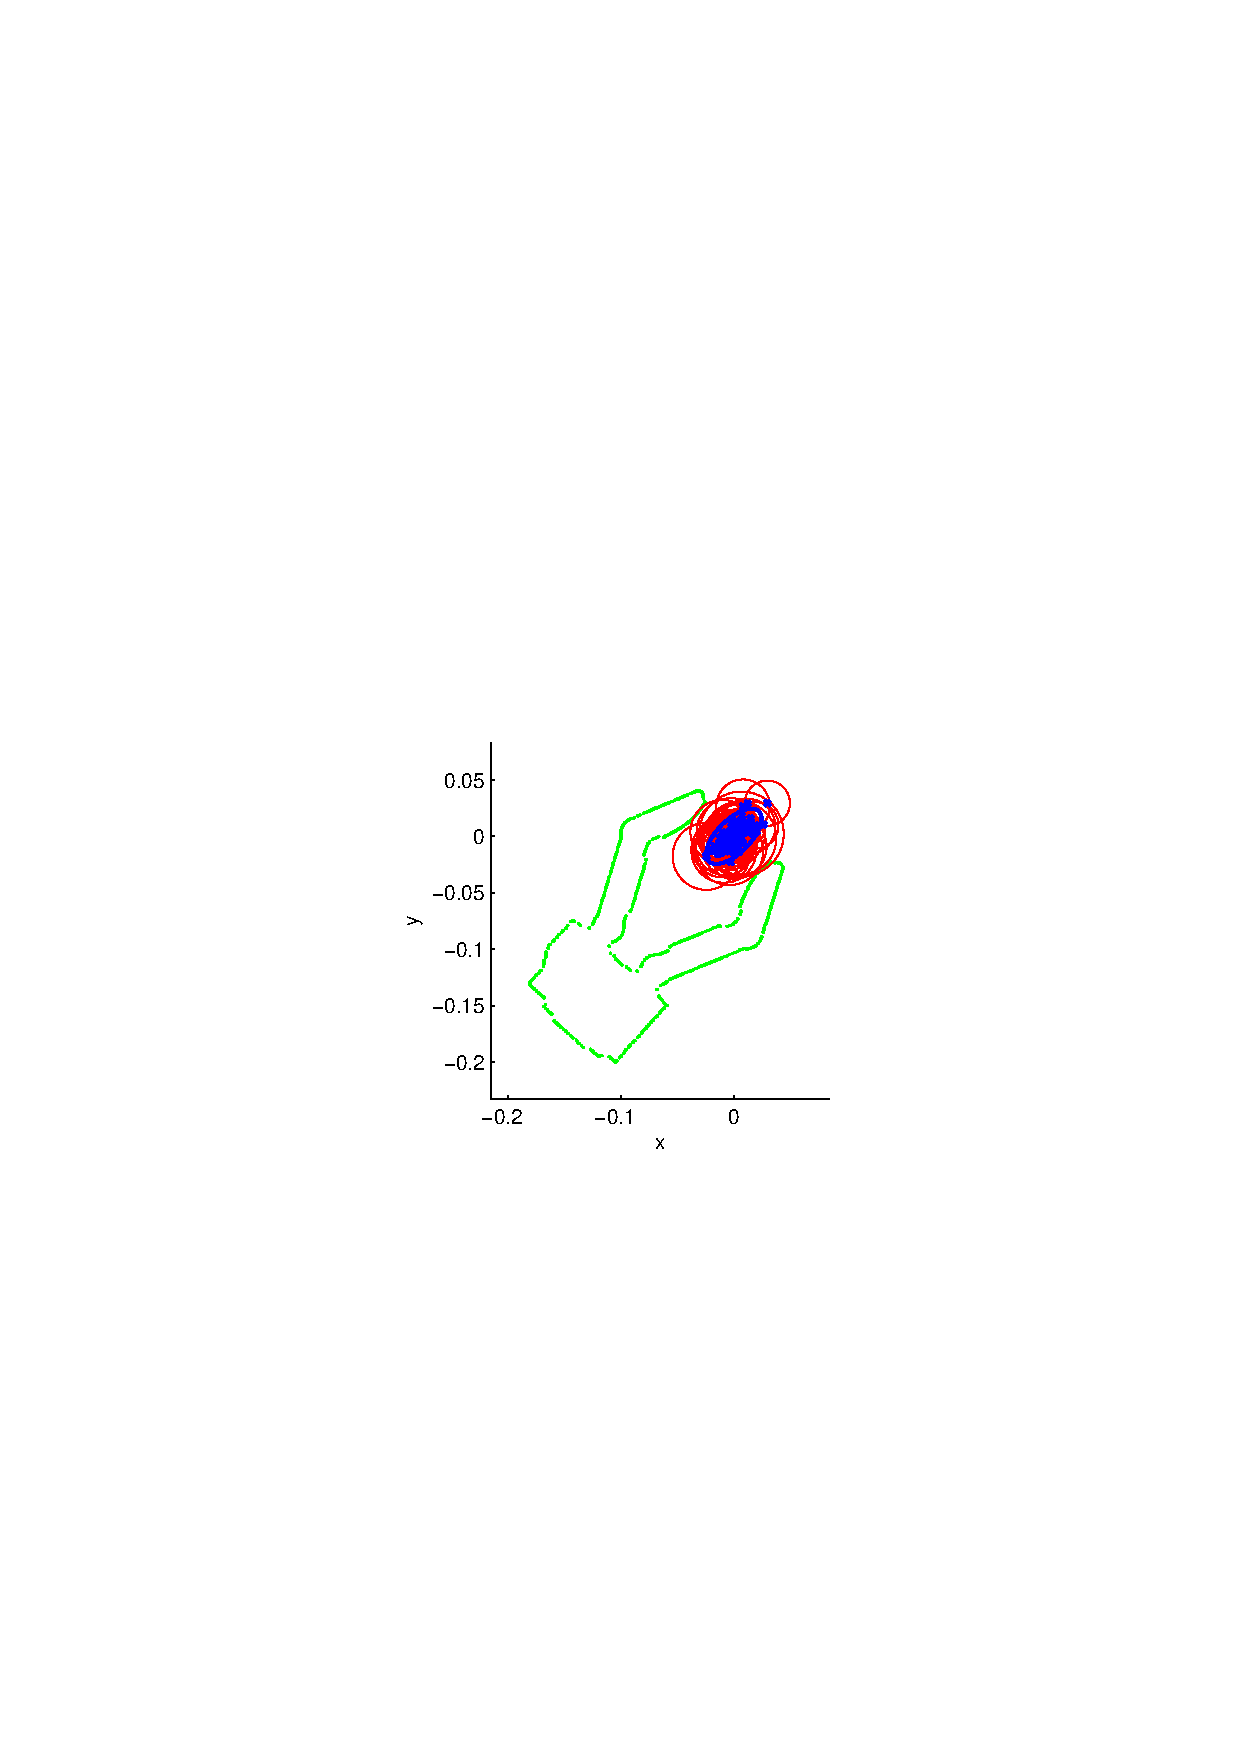
\includegraphics[width=\textwidth]{optimal_pre_touch_conf.pdf}
        \caption{The optimal pre-touch configuration computed for a circular object with the posterior shown to the left. The marginal success probability is $\text{P}(S) = 0.449$.}
        \label{fig:optimal_pre_touch_conf}
    \end{subfigure}
    \caption{An optimal pre-touch configuration computed for a given multivariate Gaussian posterior.}\label{fig:2dexample}
\end{figure}


\subsection{Experimental evaluation}
To evaluate the proposed system architecture, we performed 900 individual grasping experiments on a set of test objects. The experiments are conducted with a mobile manipulation robot. The robot's actuation system is composed of a 7 DOF KUKA LBR 4 and a 7 DOF SCHUNK SDH2 gripper mounted on top of an omnidirectional mobile base. The primary sensors of the robot are a head-mounted Kinect RGB-D camera and a hand-mounted laser time-of-flight camera (Creative Senz3D). We use the head-mounted sensor to generate the initial estimate of all objects in the scene and the hand-mounted camera for continuously tracking the target object during the grasping process.

\subsubsection{Experimental setup}
The robot is initially placed at a distance of about 1.5m from the table carrying the objects (see. Fig.~\ref{fig:setup}). At this distance, the entire table-top is in the field of view of the robot's head camera. Our purposefully delicate test objects are rolls of paper of three different radii. These test objects are very light and are easily tipped over in  the case of inaccurate grasp attempts.

We randomly select 4 test objects in each run of the experiment and place them upright on the table. The robot grasps the objects one by one, lifts them to a height of 10~cm above table and then puts them back. A grasp is considered successful if the robot manages to successfully put the test object back, so that it stands upright on the table. The latter condition enforces that the object was accurately grasped and simulates a simple manipulation operation. It follows our conviction that grasping only makes sense in a manipulation context.

\begin{figure}[!htbp]
\centering
\def\svgwidth{1\linewidth} 
%% Creator: Inkscape inkscape 0.48.4, www.inkscape.org
%% PDF/EPS/PS + LaTeX output extension by Johan Engelen, 2010
%% Accompanies image file 'experimental_setup_small.pdf' (pdf, eps, ps)
%%
%% To include the image in your LaTeX document, write
%%   \input{<filename>.pdf_tex}
%%  instead of
%%   \includegraphics{<filename>.pdf}
%% To scale the image, write
%%   \def\svgwidth{<desired width>}
%%   \input{<filename>.pdf_tex}
%%  instead of
%%   \includegraphics[width=<desired width>]{<filename>.pdf}
%%
%% Images with a different path to the parent latex file can
%% be accessed with the `import' package (which may need to be
%% installed) using
%%   \usepackage{import}
%% in the preamble, and then including the image with
%%   \import{<path to file>}{<filename>.pdf_tex}
%% Alternatively, one can specify
%%   \graphicspath{{<path to file>/}}
%% 
%% For more information, please see info/svg-inkscape on CTAN:
%%   http://tug.ctan.org/tex-archive/info/svg-inkscape
%%
\begingroup%
  \makeatletter%
  \providecommand\color[2][]{%
    \errmessage{(Inkscape) Color is used for the text in Inkscape, but the package 'color.sty' is not loaded}%
    \renewcommand\color[2][]{}%
  }%
  \providecommand\transparent[1]{%
    \errmessage{(Inkscape) Transparency is used (non-zero) for the text in Inkscape, but the package 'transparent.sty' is not loaded}%
    \renewcommand\transparent[1]{}%
  }%
  \providecommand\rotatebox[2]{#2}%
  \ifx\svgwidth\undefined%
    \setlength{\unitlength}{439.83422071bp}%
    \ifx\svgscale\undefined%
      \relax%
    \else%
      \setlength{\unitlength}{\unitlength * \real{\svgscale}}%
    \fi%
  \else%
    \setlength{\unitlength}{\svgwidth}%
  \fi%
  \global\let\svgwidth\undefined%
  \global\let\svgscale\undefined%
  \makeatother%
  \begin{picture}(1,0.50924798)%
    \put(0,0){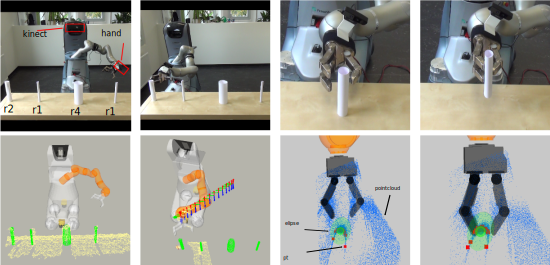
\includegraphics[width=\unitlength]{experimental_setup_small.pdf}}%
    \put(0.04104872,0.44233287){\color[rgb]{0,0,0}\makebox(0,0)[lb]{\smash{\scriptsize{Kinect}}}}%
    \put(0.18372971,0.44356854){\color[rgb]{0,0,0}\makebox(0,0)[lb]{\smash{\scriptsize{Senz3D}}}}%
    \put(0.06296952,0.30312258){\color[rgb]{0,0,0}\makebox(0,0)[lb]{\smash{\scriptsize{$\o$=2cm}}}}%
    \put(0.00 ,0.3049042){\color[rgb]{0,0,0}\makebox(0,0)[lb]{\smash{\scriptsize{$\o$=8cm}}}}%
    \put(0.12743073,0.29969816){\color[rgb]{0,0,0}\makebox(0,0)[lb]{\smash{\scriptsize{$\o$=8cm}}}}%
    \put(0.19114325,0.29981389){\color[rgb]{0,0,0}\makebox(0,0)[lb]{\smash{\scriptsize{$\o$=2cm}}}}%
    \put(0.11772753,0.00025755){\color[rgb]{0,0,0}\makebox(0,0)[lb]{\smash{(a)}}}%
    \put(0.36327459,0.00025755){\color[rgb]{0,0,0}\makebox(0,0)[lb]{\smash{(b)}}}%
    \put(0.62701032,0.00025755){\color[rgb]{0,0,0}\makebox(0,0)[lb]{\smash{(c)}}}%
    \put(0.88165172,0.00025755){\color[rgb]{0,0,0}\makebox(0,0)[lb]{\smash{(d)}}}%
    \put(0.68157634,0.16395559){\color[rgb]{0,0,0}\makebox(0,0)[lb]{\smash{\scriptsize{Point cloud}}}}%
    \put(0.5178783,0.10029525){\color[rgb]{0,0,0}\makebox(0,0)[lb]{\smash{\scriptsize{Uncertainty  ellipse}}}}%
    \put(0.51464349,0.03764591){\color[rgb]{0,0,0}\makebox(0,0)[lb]{\smash{\scriptsize{filtered points for tracking}}}}%
  \end{picture}%
\endgroup%

\captionsetup{justification=raggedright}
\caption{(a) The robot generates an initial estimate of the observed objects and their configuration parameters with the head-mounted 3D camera. This initial estimate is used to determine a pre-grasp configuration only. (b) The robot moves to the pre-grasp configuration. (c) The robot approaches the object and uses the hand-camera to continuously re-estimate object pose and radius. (d) Object is lifted up after being successfully grasped.}
\label{fig:setup}
\end{figure}	
\subsubsection{Results}
Fig.~\ref{fig:trajectory} shows the trajectory in the entire grasping process. From time 0$-$25$s$, the robot is in the pre-grasp phase in which the robot approaches the pre-grasp configuration. Approximately at time 25$s$, the pre-grasp configuration is reached and grasp motion phase begins. From then on, the \textit{grasp phase control} sends updated TCP goal configurations to the \textit{Motion adaptation} and switches from arm-platform motion to arm alone motion.
\begin{figure}[!htbp]
\centering
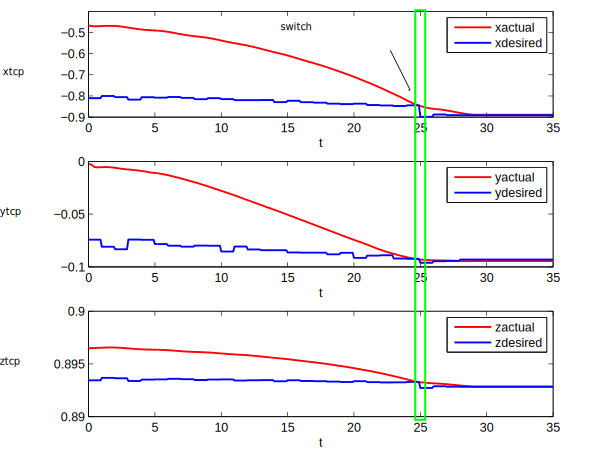
\includegraphics[width=0.8\linewidth]{trajectory.png}
\captionsetup{justification=raggedright}
\caption{Blue line is the desired TCP goal configuration. Red line is the actual trajectory of the TCP. At the 25$s$, the gripper reaches pre-grasp configuration. Grasp motion phase begins at 25$s$. In this phase the robot reactively approaches pre-touch configuration based on new sensor measurements.}
\label{fig:trajectory}       % Give a unique label
\end{figure}  

\begin{figure}[!htbp]
\centering
\includegraphics[width=0.8\linewidth]{trajectoryInxyz.png}
\captionsetup{justification=raggedright}
\caption{Illustration of the trajectory of a successful grasp}
\label{fig:demo_trajectory}       % Give a unique label
\end{figure}  
Fig.~\ref{fig:demo_trajectory} compares the originally generated reference trajectory with the actual online trajectory for a successful grasp. New TCP goals are indicated by blue circles. Two clusters of blue circles indicate goal adaptations during the entire grasping process. Comparing the distribution of blue circles, the first cluster of circles has a bigger deviation than the second cluster, because the tracking uncertainty decreases with the distance between hand-mounted 3d camera and the target object. Besides that, the motion control errors of the mobile platform during the first phase also contribute to the deviation of the first cluster. 

We compare our approach with two other traditional approaches. Since our approach both considers uncertainty and grasp adaptation, we regard our approach as `closed-loop uncertainty-aware'. Both other approaches execute grasping in a open-loop fashion. The entire grasping trajectory is pre-computed at the pre-grasp configuration. One approach uses the same uncertainty-aware method proposed to compute the pre-touch configuration, while the other method compute the pre-touch configuration by sampling a random approach direction. The experiment is repeated 100 times for each object with different radius. In total, 900 grasp outcomes are recorded. Fig.~\ref{fig:exp_result} shows the experimental results. Our closed-loop uncertainty-aware approach achieves an average success rate of over 90 $\%$ regardless of actual object size, while the success rate of other two approaches are dependent on the size. For smaller objects ($\o=2$cm, $\o=4$cm) they often missed the objects or hit the objects while approaching the pre-touch configuration. Comparing both open-loop approaches, explicitly considering the uncertainty also contributes to the overall grasping success, because the uncertainty-aware approach generates the pre-touch configuration with higher marginal success probability. The accompanying video attachment depicts the entire grasping process with different methods used in this experiment. In summary, both closed-loop control and uncertainty-awareness are key factors to achieve a robust grasping performance. 

\begin{figure}[!htbp]
\centering
\includegraphics[width=0.8\linewidth]{graspsuccessrate.png}
\captionsetup{justification=raggedright}
\caption{Comparison of grasp success rate between methods. In total, 900
grasp trials were performed to obtain the data.}
\label{fig:exp_result}       % Give a unique label
\end{figure} 

\begin{figure}
    \centering
    \begin{subfigure}[t]{0.45\textwidth}
        \includegraphics[width=\textwidth]{fail1.png}
        \caption{This figure shows a typical grasping failure using the open-loop uncertainty-aware approach. The object is tipped over during the force-closure phase because the desired pre-touch configuration is not actually reached during the grasp motion phase. Uncertain perception and execution lead to this failure.}
        \label{fig:failed_grasp_1}
    \end{subfigure}
    ~ %add desired spacing between images, e. g. ~, \quad, \qquad, \hfill etc. 
    \begin{subfigure}[t]{0.45\textwidth}
        \includegraphics[width=\textwidth]{fail2.png}
        \caption{This figure shows another grasping failure when using the open-loop random approach direction method. The grasp fails, because the fingers were closed at the wrong place. Randomly chosen approaching direction occasionally generates a longer trajectory which introduces uncertainty in actuation.}
        \label{fig:failed_grasp_2}
    \end{subfigure}    
\end{figure}

\section{Summary}
In this chapter, we address the problem of how to make grasp execution more robust. For this purpose, we propose an adaptive whole body control architecture specific tailored for mobile manipulators. Our control architecture contains seven major modules which close the entire loop from perception to control. We specifically focus on the reach-to-grasp phase, in which the gripper of a robot moves from a `pre-grasp' configuration towards the final grasp configuration. Different from the traditional methods which execute grasps in open loop, our method allows vision feedback to be continuously integrated. We exploit dynamic movement primitives for online trajectory adaptation. In this way, the robot continuously reduces the uncertainty during the grasping process. It allows a robust execution even the perceptual uncertainty could be large at the beginning of the process.   

Another advantage of our architecture is the flexibility of coordinating different actuators to perform a certain motion. Our robot imitates how humans coordinate their locomotion, torso, arm and hand to grasp objects. We exploit arm-platform coordination and arm-gripper coordination for mobile manipulators. The arm-platform keeps the gripper in a `good' configuration that the manipulability of the arm is maximized. In the case of grasping objects from the top, the arm-gripper coordination can keep the fingers of a gripper in contact with a support surface to increase the chance of success. 

We evaluate the proposed architecture in a challenging grasp scenario. The object that we choose for the experiment is difficult to grasp, because of its weight and place orientation. The sensor we used to perform this task contains large noise which even more increase the difficulty. We combine the uncertainty-aware grasp synthesis which we proposed in the earlier chapter and demonstrate that considering uncertainty as well as closed-loop grasp execution significantly increase the grasp success.

